\subsection{Kỹ thuật Full Scan DFT (Full Scan DFT Technique)}
Với kiến thức nền từ Phần 7.2, ta tiến tới thảo luận các tiêu chuẩn thực hành DFT phổ biến nhất, đó là quét toàn phần (Full scan). Kỹ thuật này có ý tưởng tương tự với "Isolated serial scan" nhưng giúp giải quyết vấn đề bằng cách tích hợp luôn thanh ghi dịch vào trực tiếp các flip-flop trạng thái của mạch (state flip-flops). Việc này vừa giảm tối đa chi phí phần cứng cồng kềnh, vừa biến CUT (mạch cần kiểm thử) trên nền tảng tuần tự trở thành một mạch hoàn toàn mang tính tổ hợp (combinational circuit).

\begin{figure}[H]
    \centering
    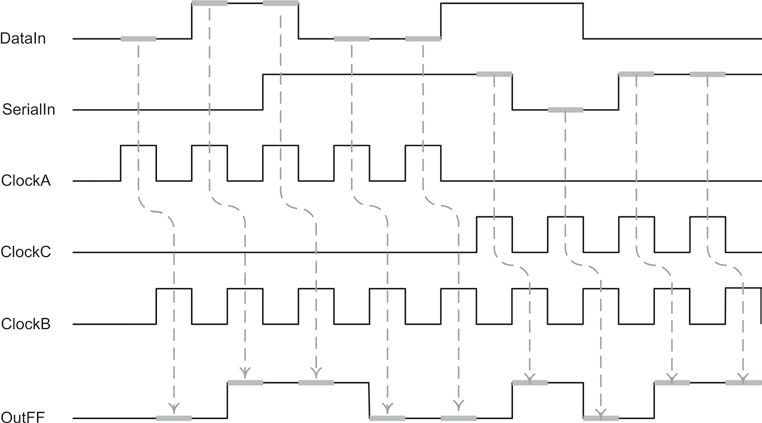
\includegraphics[width=0.7\textwidth]{images/FullScanDftTechnique.png}
    \caption{\textit{Kỹ thuật Full scan DFT (Full scan DFT technique)}}
\end{figure}

\subsubsection{Chèn Full Scan (Full Scan Insertion)}

\begin{figure}[H]
    \centering
    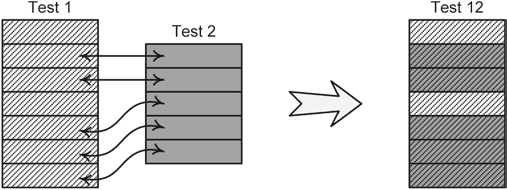
\includegraphics[width=0.7\textwidth]{images/ScanInsertion.png}
    \caption{\textit{Chèn Scan (Scan insertion)}}
\end{figure}

\begin{figure}[H]
    \centering
    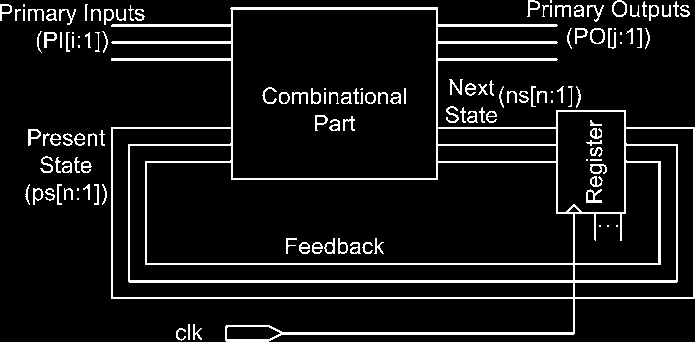
\includegraphics[width=0.7\textwidth]{images/TestableHuffmanModelFeedbackRegister.png}
    \caption{\textit{Thanh ghi phản hồi mô hình Huffman có thể kiểm thử}}
\end{figure}

\paragraph{Thanh ghi Scan}
Để chèn scan, ta bắt đầu với mô hình tuần tự của Huffman. Quá trình Full scan biến các phần cứng của mô hình thay đổi. Phần thanh ghi của mô hình Huffman lúc này bao gồm cả chế độ dịch nối tiếp tín hiệu đầu vào \texttt{STDI} (Serial Test Data In) vào trong thanh ghi dịch, và luân phiên nạp dữ liệu song song ở chế độ bình thường.
Trong chế độ kiểm thử, \texttt{NbarT} bằng 1, thanh ghi trở thành thanh ghi dịch. Ở chế độ bình thường, \texttt{NbarT} bằng 0 và giá trị trạng thái kế tiếp (ns) được nạp vào trạng thái hiện tại (ps).

\begin{lstlisting}[language=Verilog, caption={Mô hình thanh ghi phản hồi thử nghiệm kiểu Huffman}]
module FBRegister #(parameter size = 4) (
    input [size-1:0] ns, 
    input STDI, Clock, NbarT, Reset, 
    output STDO,
    output reg [size-1:0] ps
);
    always @(posedge Clock) begin
        if (Reset == 1'b0 ) begin
            if (NbarT == 1'b0) ps <= ns; 
            else ps <= {STDI, ps[size-1:1]}; // Chế độ Shift
        end
        else
            ps <= 0;  
    end
    assign STDO = ps[0] ;
endmodule
\end{lstlisting}

\paragraph{Quy trình kiểm thử}
Quy trình chỉ liên quan đến phần tổ hợp. Cấu trúc thử nghiệm tạo đầu vào giả (PPI) ở ps và đầu ra giả (PPO) ở ns. Với chế độ thử nghiệm (\texttt{NbarT}=1), dữ liệu được dịch dần vào trong thanh ghi. Sau khi dịch xong toàn bộ bit, phần thứ nhất của dữ liệu đã sẵn sàng trên chân vào ps. Phần thứ hai của dữ liệu kiểm thử được đặt lên các pin vật lý (PI). Mạch tổ hợp sẽ truyền giá trị qua và đưa ra thiết bị phân tích lưu trữ. Sau đó, ta tắt mạch về chế độ thường (\texttt{NbarT}=0), và cấp duy nhất 1 nhịp đồng hồ, đẩy ns vào thanh ghi song song. Bước cuối cùng, PPO được dịch ra đồng thời với chu trình nạp mới của Test.

\subsubsection{Cấu trúc Flip-flop (Flip-flop Structures)}
Ở trên ta đã mô phỏng một thanh ghi scan với NbarT. Có những cấu trúc giúp tiết kiệm độ trễ hoặc cổng logic hơn trên thực tế.

\begin{figure}[H]
    \centering
    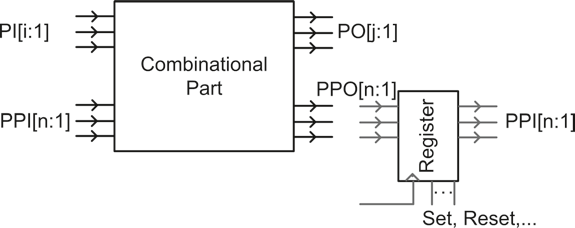
\includegraphics[width=0.7\textwidth]{images/BasicLatch.png}
    \caption{\textit{Chốt cơ bản (Basic latch)}}
\end{figure}

\begin{figure}[H]
    \centering
    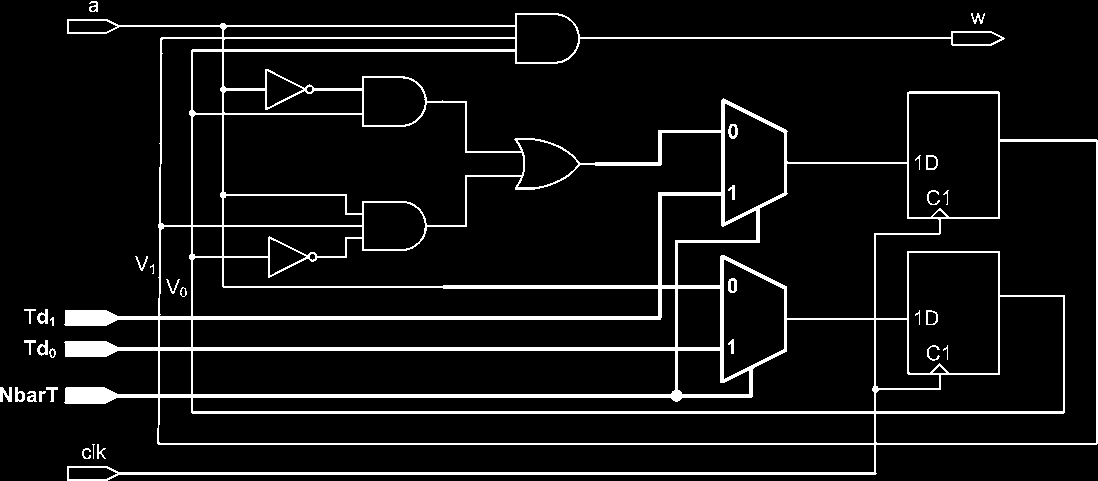
\includegraphics[width=0.7\textwidth]{images/DLatch.png}
    \caption{\textit{Chốt loại D (D-latch)}}
\end{figure}

\begin{figure}[H]
    \centering
    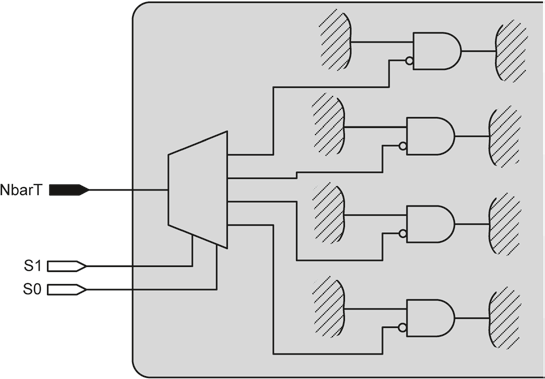
\includegraphics[width=0.7\textwidth]{images/CmosLatches.png}
    \caption{\textit{Chốt CMOS (CMOS latches)}}
\end{figure}

\begin{figure}[H]
    \centering
    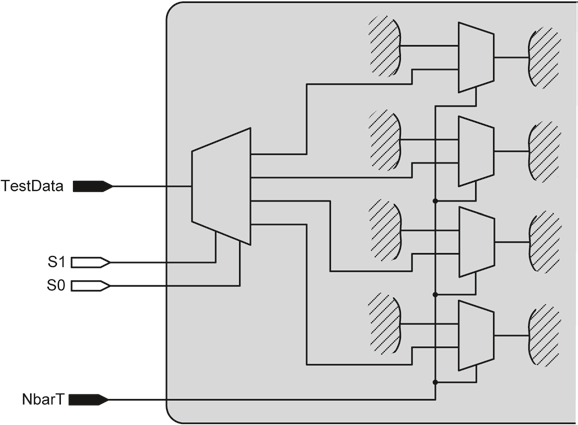
\includegraphics[width=0.7\textwidth]{images/DTypeFlipFlop.png}
    \caption{\textit{D-type flip-flop}}
\end{figure}

\paragraph{Dữ liệu kiểm thử dồn kênh (Multiplexed Test Data)}
Flip-flop kèm bộ phận Multiplexer dùng NbarT để chọn lựa: khi 0 thì thu \texttt{DataIn}, khi 1 thì thu nối tiếp \texttt{SerialIn}. Đầu ra bị đảo dồn thành thao tác Reset. Dưới đây là mã Verilog của phần tử cực kì phổ biến này:

\begin{figure}[H]
    \centering
    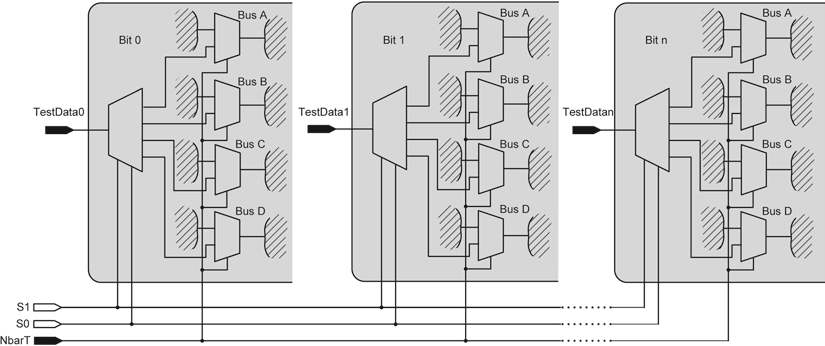
\includegraphics[width=0.7\textwidth]{images/MultiplexedScanElement.png}
    \caption{\textit{Phần tử quét dồn kênh (Multiplexed scan element)}}
\end{figure}

\begin{figure}[H]
    \centering
    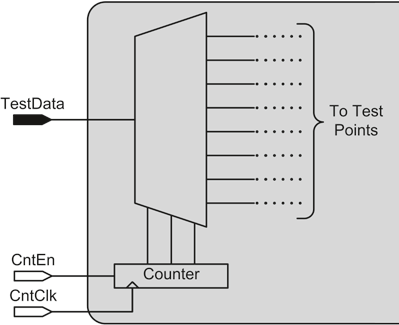
\includegraphics[width=0.7\textwidth]{images/ScanRegisterMultiplexedFlipFlops.png}
    \caption{\textit{Thanh ghi quét với các flip-flop dồn kênh}}
\end{figure}

\begin{lstlisting}[language=Verilog, caption={Cấu trúc Muxed Scan Flip-Flop (Hình 7.25)}]
module MuxedFF (
    input NbarT, Reset, DataIn, SerialIn, Clock, 
    output reg OutFF
);
    always @(negedge Clock) begin
        if (Reset) OutFF <= 1'b0;
        else OutFF <= ~NbarT ? DataIn : SerialIn;
    end 
endmodule
\end{lstlisting}
Vấn đề với thiết kế này là trễ logic tăng lên vì tín hiệu bị chèn ép qua Multiplexer ngay cửa ngõ D của Flip-flop, khiến tốc độ mạch tổng thể bị chậm đi ở chế độ hoạt động bình thường.

\paragraph{Hệ thống xung nhịp kép (Dual Clocking)}
Vì delay của test chỉ cần qua shift-register ngắn ngủi mà không cần qua mạch tổ hợp phức tạp, ta có thể đổi sử dụng một Clock cực nhanh riêng biệt cho thao tác test data (TestClock). Flip-flop với Dual Clock sử dụng logic OR để trộn \texttt{DataClock} và \texttt{TestClock}. Dù linh hoạt nhưng mạch này dễ bị hiện tượng hazard tại chân D của flip-flop.

\begin{figure}[H]
    \centering
    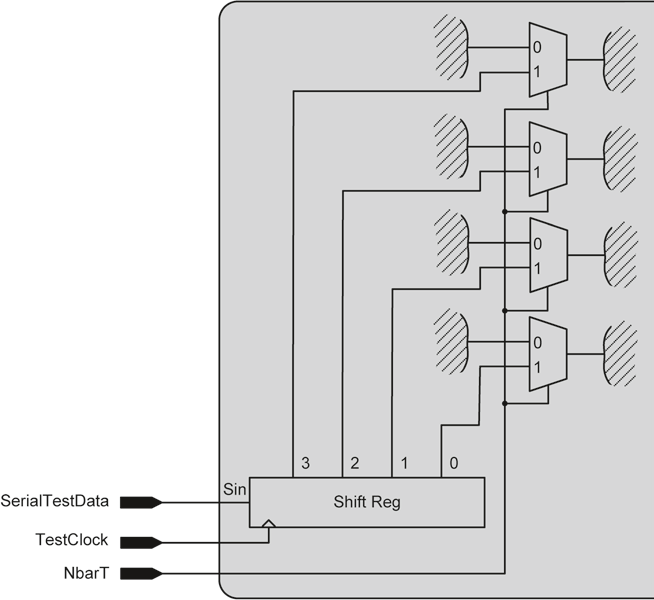
\includegraphics[width=0.7\textwidth]{images/ScanFlipFlopDualClocking.png}
    \caption{\textit{Scan flip-flop với xung nhịp kép (Dual clocking)}}
\end{figure}

\begin{lstlisting}[language=Verilog, caption={Dual Clock Scan Flip-Flop (Hình 7.27)}]
module DualClockFF (
    input DataIn, DataClock, SerialIn, TestClock, 
    output reg OutFF
);
    wire Clock = DataClock | TestClock;
    always @(negedge Clock) begin
        if (DataClock) OutFF <= DataIn;
        else if (TestClock) OutFF <= SerialIn;
    end
endmodule
\end{lstlisting}

\paragraph{Flip-flop Hai Cổng (Two-port Flip-flops)}
Để không làm trễ phần cổng D mà vẫn tách xung nhịp, cấu trúc 2 port với LSSD (Level Sensitive Scan Design - thiết kế rất nổi tiếng từ IBM) bao gồm 2 latch (master/slave). Việc đọc song song dùng \texttt{ClockA} và \texttt{ClockB}, còn chế độ kiểm thử thì dùng luân phiên \texttt{ClockC} và \texttt{ClockB}.

\begin{figure}[H]
    \centering
    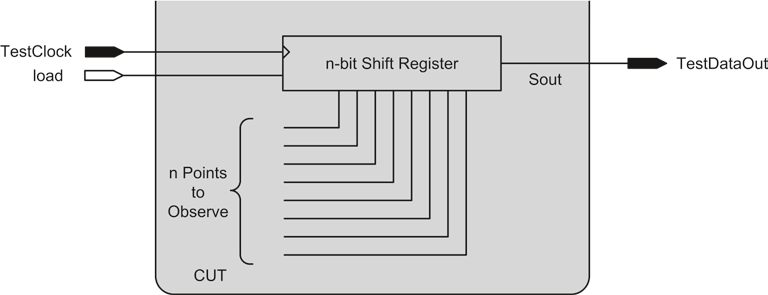
\includegraphics[width=0.7\textwidth]{images/TwoPortThreeClockFlipFlop.png}
    \caption{\textit{Flip-flop hai cổng ba xung nhịp}}
\end{figure}

\begin{figure}[H]
    \centering
    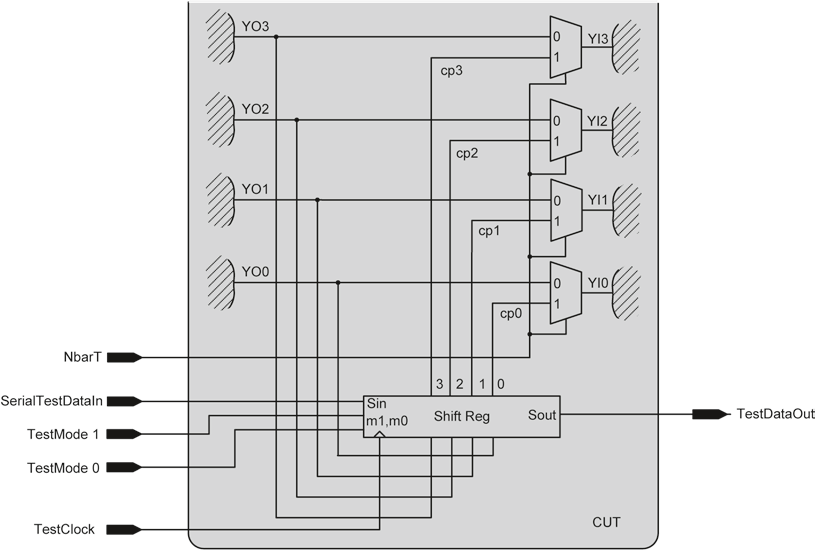
\includegraphics[width=0.7\textwidth]{images/TwoPortFlipFlopTiming.png}
    \caption{\textit{Định thời flip-flop hai cổng}}
\end{figure}

\begin{figure}[H]
    \centering
    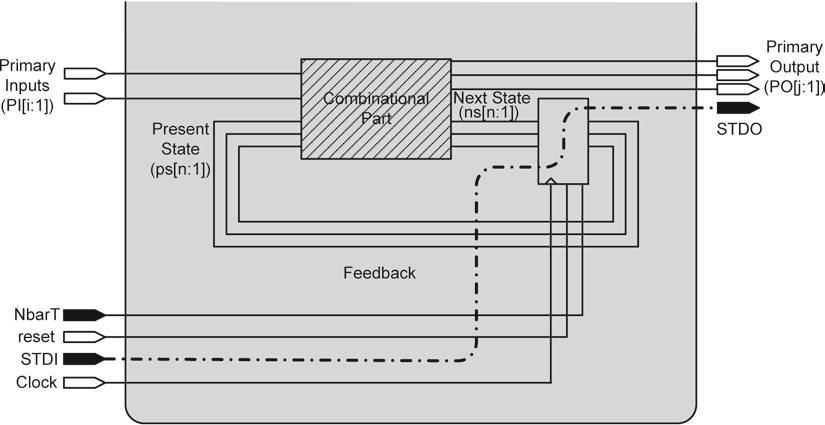
\includegraphics[width=0.7\textwidth]{images/LssdDesign.png}
    \caption{\textit{Thiết kế LSSD}}
\end{figure}

\subsubsection{Thiết kế và Kiểm thử Full Scan (Full Scan Design and Test)}
Toàn bộ quá trình chuẩn bị cấu trúc full scan từ RTL tới tester ảo bao gồm 7 bước. Lấy ví dụ mạch đếm Residue-5 (được nhắc ở các chương trước) được thiết kế bằng mô hình tuần tự:
\begin{enumerate}
    \item \textbf{Thiết kế và Giám định (Design Validation):} Đảm bảo chức năng gốc chạy hoàn hảo trên testbench (testbench migration).
    \item \textbf{Tổng hợp sơ đồ Netlist:} Mã Verilog RTL biên dịch thành một loạt cổng AND, OR thông qua tổng hợp FPGA thành netlist chuẩn (với output \texttt{out\_0}, \texttt{out\_1}, ...). Tín hiệu clock cấp cho hệ logic flip-flop DFF.
    \item \textbf{Trải phẳng (Unfolding):} Cắt đứt thanh ghi phản hồi. Đổi cực nối mạch để input của DFF chuyển thành Pseudo Primary Output (PPO) và output của DFF thành Pseudo Primary Input (PPI). Hệ tuần tự lúc này vỡ thành hệ tổ hợp.
    \item \textbf{Khởi chạy Phần mềm tạo thử nghiệm tổ hợp (Combinational TPG):} Do hệ đã hóa tổ hợp, chạy Tool để sinh vectơ test. Ví dụ: Tool tìm ra 104 lỗi, tạo 26 mẫu test vector hoàn hảo bao phủ 100\% (Fault coverage = 100\%). Nếu chạy tuần tự với độ khó cũ, độ bao phủ chỉ được 82.4\%.
    \item \textbf{Chèn mạch Scan thật (Scan Insertion):} Bắt đầu nối tiếp chân xuất nối tiếp (So) sang ngõ vô tín hiệu lối tiếp của tầng kia bằng các \texttt{Si} và điều khiển chung bởi cờ \texttt{NbarT}.
    \item \textbf{Xây dựng bộ kiểm thử ảo (Virtual Tester):} Một "Automated test equipment - ATE" thông qua phần mềm Testbench đọc từ mô-đun tệp dữ liệu test (test data file). Đồng thời tự chèn những lỗi ngẫu nhiên trong phần code để xem chuỗi 26 vectors này có túm gọn được mớ lỗi đó hay không.
\end{enumerate}

\begin{figure}[H]
    \centering
    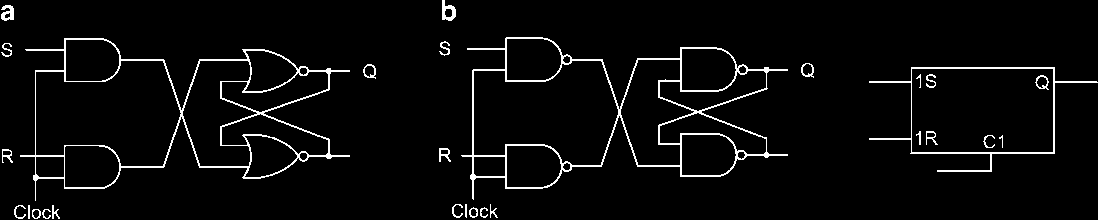
\includegraphics[width=0.7\textwidth]{images/PostsynthesisResidue5Netlist.png}
    \caption{\textit{Netlist residue5 sau tổng hợp (Postsynthesis)}}
\end{figure}

\begin{figure}[H]
    \centering
    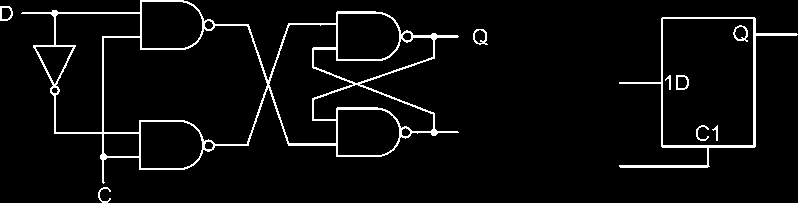
\includegraphics[width=0.7\textwidth]{images/UnfoldedResidue5Netlist.png}
    \caption{\textit{Netlist residue5 trải phẳng (Unfolded)}}
\end{figure}

\begin{figure}[H]
    \centering
    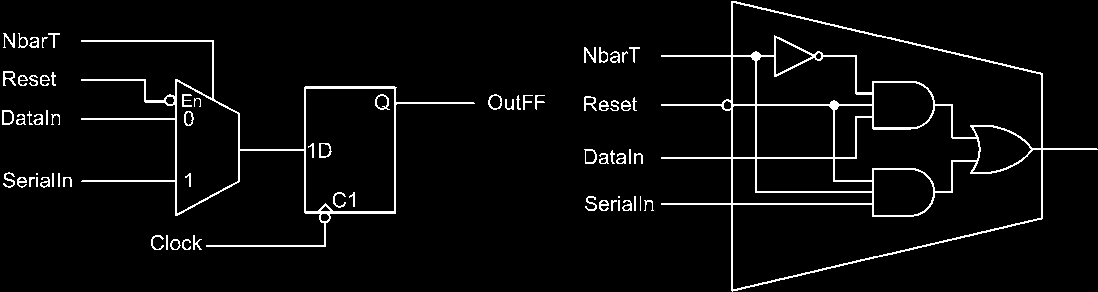
\includegraphics[width=0.7\textwidth]{images/Residue5ScanChain.png}
    \caption{\textit{Chèn chuỗi quét (Scan chain) cho residue5}}
\end{figure}

\begin{figure}[H]
    \centering
    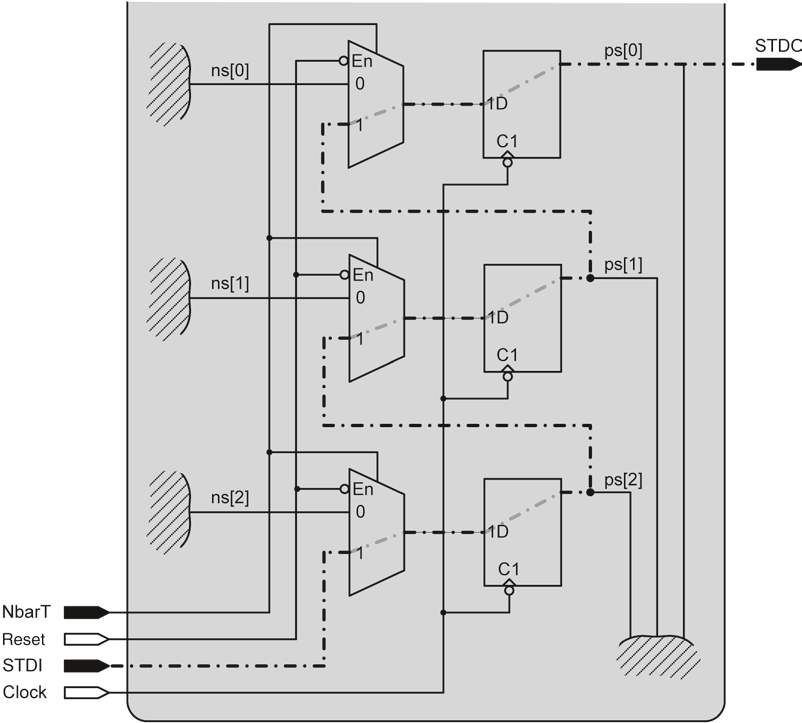
\includegraphics[width=0.7\textwidth]{images/VirtualTesterFullScanResidue5.png}
    \caption{\textit{Virtual tester cho phần full scan Residue-5}}
\end{figure}

\begin{lstlisting}[language=Verilog, caption={Trích xuất chương trình Virtual Tester chèn lỗi kiểm thử scan chain}]
module Tester;
    res5_ScanInserted FUT(clk, reset, PI, PO, NbarT, si, so); 
    always #10 clk = ~clk;
    initial begin 
        while( !$feof(faultFile)) begin
            status = $fscanf (faultFile,"%s s@%b\n",wireName, stuckAtVal);
            $InjectFault (wireName, stuckAtVal); // Giả lập lỗi
            global_reset = 1'b1; reset = 1'b1; #1;
            global_reset = 1'b0; reset = 1'b0; 
            while((!$feof(testFile))&&(!detected) ) begin
                // Tải vector, tiến trình đọc và kích hoạt test
            end
            if(detected == 0) $display ("NOT DETECTED = %s s@%b", wireName, stuckAtVal);
            $RemoveFault(wireName); // Phục hồi sau kiểm tra
        end
        $stop;
    end
endmodule
\end{lstlisting}

\begin{figure}[H]
    \centering
    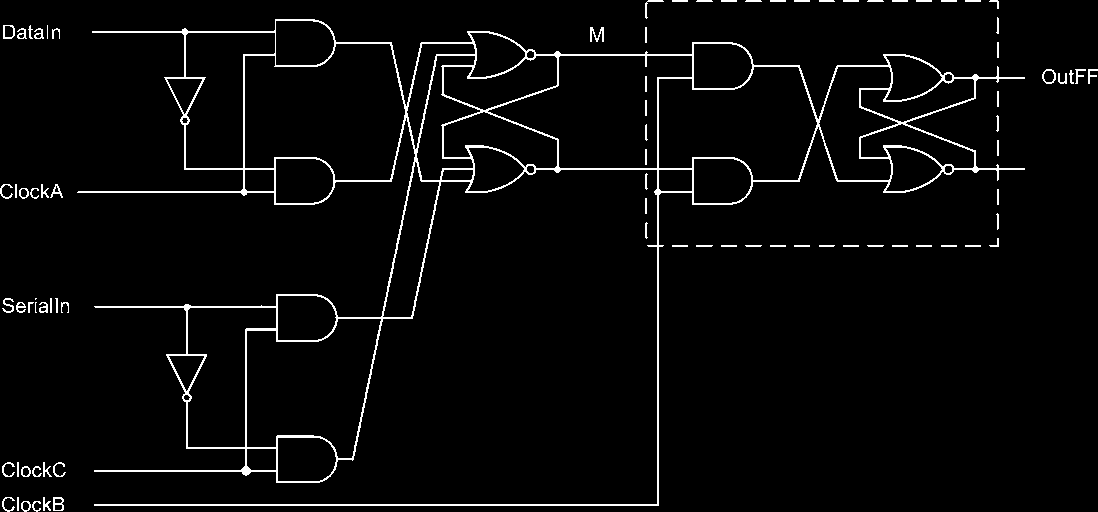
\includegraphics[width=0.7\textwidth]{images/TestApplicationResponseCollection.png}
    \caption{\textit{Áp dụng kiểm thử và thu thập phản hồi (Test application and response collection)}}
\end{figure}
